\subsection{Active Optics System Commissioning}
\label{sec:aos_commissioning}

AOS commissioning started on 2024-10-24 with the first ComCam images delivering a remarkable 1.7 arcsecond
full-width half-maximum (FWHM) image quality. At the end of the campaign we had shown that we could align the
telescope optics, determine and correct for optical aberrations using the hexapods and bending modes for M2
and M1M3, and apply these corrections as a closed loop system. For some of the observations we met the image
quality requirements of the LSST system (\ie with the optical system delivering less than 0.4 arcseconds to
the image quality budget) but there are still significant challenges in delivering seeing limited images
consistently in all observing conditions.

Sub-arcsecond image quality was first achieved on the night of 2024-11-06, with a best image quality of 0.66 arcsecond FWHM (with a 0.1 arcsecond variation across the field achieved) on the night of 2024-11-12 in $z$. The AOS system was able to achieve closed-loop corrections using wavefront estimation across varying elevations and stellar densities. Closed-loop operations have been run autonomously by the observing specialists to show that the scripts and procedures are mature. Preparations are underway to prototype a fully autonomous survey-mode triplet-taking block before the conclusion of ComCam's on-sky operations.

While we have demonstrated that Rubin can achieve the optical performance requirements for the AOS system there are significant challenges in meeting the optical performance requirements consistently as a function of temperature and elevation. It is not currently clear which aspects of the optical system are limiting its performance but the AOS team is working to understand the source of high levels of defocus and some amount of astigmatism that are present in the Zernike measurements. The team is also working to improve the computational efficiency of the system, which currently takes 5 minutes to complete a closed-loop iteration. 

The AOS algorithms appear robust for a range of source densities and image qualities. A number of failure modes of the AOS software are present and being investigated. These include failures in processing images through Rapid Analysis when donuts cannot be detected on all sensors, and difficulty in measuring the wavefront when the images are significantly defocused (e.g., when the intra or extra focal images appear in focus). The AOS team is working to improve the robustness of the system to monitor these and other failure modes.

\figRef{aos} shows the FWHM delivered by the optical system (black line) as we correct the alignment
and bending modes of the mirrors and camera over the nights 2024-11-25 to 2024-12-01. The FWHM is estimated
from the Zernike amplitudes measured from out-of-focus donuts. The grey and blue lines are the 500nm and
zenith corrected image qualities measured by the SOAR \RINGSS seeing monitor and from the Rubin images
respectively. The dashed green line is the 0.25 arcseconds image quality requirement for the telescope
optics. From these measurements the AOS system is shown to be capable of meeting the image quality requirements.

\begin{figure}
    \centering 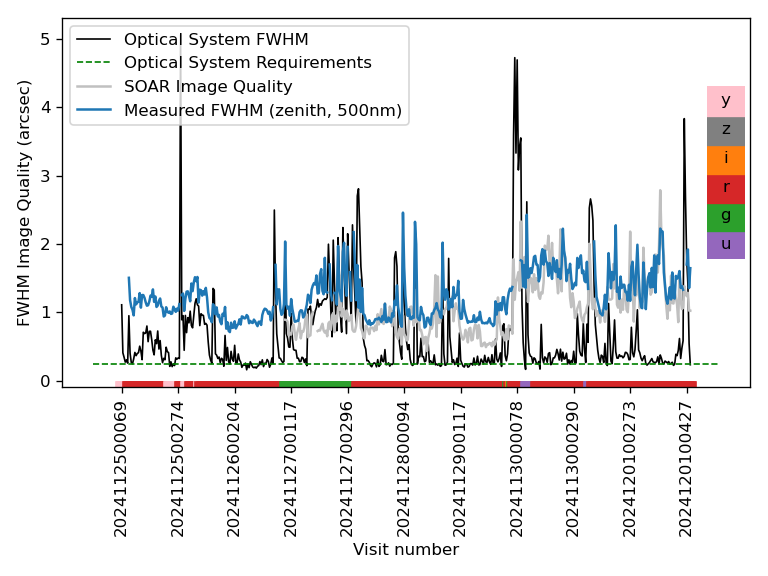
\includegraphics[width=0.7\textwidth]{figures/optical_performance.png}
    \caption{The FWHM delivered by Rubin (blue), the image quality from Rubin's optical system estimated from the AOS (black), and the  image quality measured by SOAR (gray). The Rubin and SOAR measured FWHMs are corrected to 500nm and zenith.}
    \label{fig:aos}
\end{figure}

%z22 z11

\subsubsection{Initial Alignment}
Initial alignment of the AOS utilizes an updated laser tracker nominal frame based on a Final Element Analysis
Model to ensure that the system is brought into focus prior to the start of observations.  Combined with a
measurement of the impact of gravity on the telescope, these refinements simplified the alignment process,
demonstrating the value of accurate laser tracker data. Once we were able to get on-sky images using curvature
wavefront sensing, we finalized the initial state of the hexapods position to ensure a well aligned system at
the start of each night. Work is ongoing to understand the stability of the initial hexapod and bending mode positions across nights to determine how well we can predict the  configuration of the AOS system at the start of each night. 


\subsubsection{Wavefront estimation}
The wavefront estimator proved robust across diverse observing conditions of seeing, mount elevation and a few filters (r,i and y band) 
On dense fields such as 47 Tuc or NGC 253, the estimator provided accurate results for  all sensors except the central one.  Comparison of observed PSFs with simulations  confirmed the  accuracy of Rubin's ray-tracing software, \Batoid.

Wavefront estimation and closed-loop convergence has been demonstrated using \texttt{TIE} and \texttt{Danish}. Other advancements include the implementation of sparse Zernikes,  allowing selective inclusion of Zernike polynomial terms while minimizing cross-contamination 
of modes with identical azimuthal dependencies.

Despite delivering good optical quality, Zernike measurements indicate persistently high levels of defocus and some amount of astigmatism. We are continuing to investigate the source and impact of these measurements.

\subsubsection{Closed Loop}
Following resolution of initial issues with the AOS pipelines,  closed-loop operations were achieved across varying elevations and filters ($u$, $g$, $r$, $i$, $z$, and $y$).  Most optical modes were utilized, excluding the three highest-order modes on M2.  Consistency in results across nights confirmed the need for further refinement of the LUT. In favorable seeing conditions, the system achieved sub-arcsecond image quality, with FWHM as low as 0.65 arcseconds.

The closed loop process still takes 5min  often requiring 5 or more iterations. The best performance for the closed loop achieved convergence in two iterations but delivering this consistently has not been achieved and tuning the closed-loop gain and making further adjustments to improve computational  efficiency remains a priority for the team.

\subsubsection{LUT}
The LUT underwent initial validation across elevations, azimuths, and rotator angles, 
leading to incremental improvements. While these updates enhanced performance, 
further refinements are needed to address second-order dependencies. Insights 
from ComCam data will inform these efforts, ensuring readiness for LSSTCam, which 
may present distinct challenges due to its larger focal plane and optical system.

\subsubsubsection{Next Steps}
\begin{itemize}
\item
  Conduct step-by-step closed-loop validations for LSSTCam, validating signs and rotations for intentional perturbations.
\item
  Collaborate with the Camera Team to anticipate and mitigate known camera tilts.
\item
  Implement and validate tests tailored to LSSTCam's larger focal plane dimensions.
\item
  Prepare RubinTV and donutViz for full-array LSSTCam mode and automate its execution for all triplet-taking sequences.
\item
  Adapt MTAOS to run as a continuous background task, supporting survey-mode operations.
\item
  Optimize the AOS pipeline for speed, including binning and ISR performance improvements.
\end{itemize}

